% fig-opcost: deployment economics (2x2)
% Data: R/opcost_*.csv → out/opcost-panel-[a-d].tex
\documentclass[border=2pt]{standalone}
% inspect_style.tex: Shared style definitions for all Inspect figures
% Enforces uniform fonts, colors, and panel label positioning

\usepackage[T1]{fontenc}
\usepackage{lmodern}  % Latin Modern for Type 1 fonts
\usepackage{amssymb}  % \blacksquare for shared legends
\usepackage{pgfplots}
\usepackage{pgfplotstable}
\pgfplotsset{compat=1.18}

% Color palette (Okabe-Ito colorblind-safe, print-safe)
% -- Backbones (used wherever PatchCore vs Dinomaly are distinguished)
\definecolor{cPatchcore}{HTML}{0072B2}   % blue
\definecolor{cDinomaly}{HTML}{D55E00}    % vermillion
% -- Decision classes / gates
\definecolor{cAccept}{HTML}{009E73}      % green
\definecolor{cDefer}{HTML}{E69F00}       % orange
\definecolor{cReject}{HTML}{D55E00}      % red
\definecolor{cControl}{HTML}{56B4E9}     % light blue
\definecolor{cTransfer}{HTML}{CC79A7}    % pink
% -- Benchmarks (canonical palette; used wherever MVTec/VisA/MPDD are
%    distinguished, so benchmark colouring is uniform across all figures and
%    never collides with the backbone blue/vermillion above)
\definecolor{cMVTecAD}{HTML}{0072B2}     % blue
\definecolor{cVisA}{HTML}{E69F00}        % orange
\definecolor{cMPDD}{HTML}{009E73}        % green

% Typography defaults
\newcommand{\figfont}{\fontsize{8}{9.5}\selectfont}
\newcommand{\axislabelfont}{\fontsize{9}{10}\selectfont}
\newcommand{\titlefont}{\fontsize{9}{10}\selectfont}
\newcommand{\tickfont}{\fontsize{7}{8}\selectfont}
\newcommand{\panellabelfont}{\fontsize{9}{10}\selectfont\bfseries}

% Panel label OUTSIDE the axis (axis clip would otherwise swallow it).
% Usage after \end{axis}: \panellabel{axname}{a}
% Parked in the left gutter at the top of the axis frame — NOT on the
% title baseline — so titles can stay truly centered over the plot box.
\newcommand{\panellabel}[2]{%
  \node[anchor=south east, font=\panellabelfont, inner sep=0.5pt]
    at ([xshift=-8pt, yshift=7pt] #1.north west) {\textbf{#2}};%
}

% Standard axis styles. Titles centered above the plot box only.
\pgfplotsset{
  inspect/centertitle/.style={
    title style={at={(0.5,1.10)}, anchor=south, font=\titlefont},
  },
  inspect default/.style={
    axis x line=bottom,
    axis y line=left,
    xlabel style={font=\axislabelfont},
    ylabel style={font=\axislabelfont},
    inspect/centertitle,
    x tick label style={font=\tickfont},
    y tick label style={font=\tickfont},
    legend style={font=\tickfont, draw=none, fill=none},
  }
}


\definecolor{cGate}{HTML}{0072B2}
\definecolor{cBase}{HTML}{D55E00}

\begin{document}
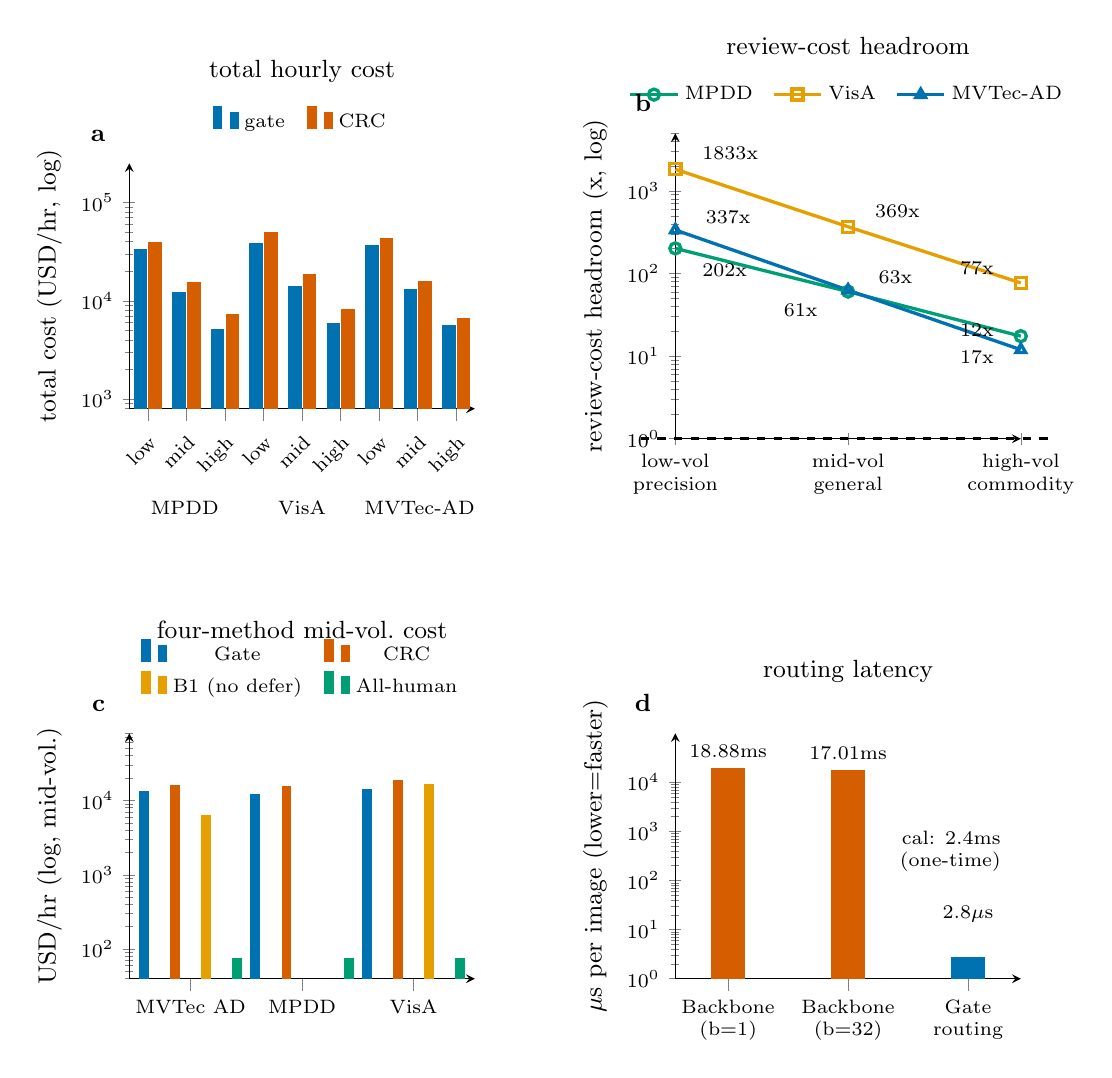
\begin{tikzpicture}[font=\figfont]

% Panel a: total cost grid
\begin{axis}[
  inspect default,
  name=axa, width=2.35in, height=1.85in, at={(0.42in,2.85in)},
  ymode=log, ymin=800, ymax=250000,
  ylabel={total cost (USD/hr, log)},
  xtick={0,1,2,3,4,5,6,7,8},
  xticklabels={low,mid,high,low,mid,high,low,mid,high},
  x tick label style={font=\tickfont, rotate=45, anchor=north east},
  ybar=0.8pt, bar width=4.5pt,
  enlarge x limits=0.06,
  % Horizontal legend above the plot box so it never collides with panel letter a.
  legend style={at={(0.5,1.08)}, anchor=south, legend columns=2, font=\tickfont, draw=none,
    /tikz/every even column/.append style={column sep=6pt}},
  title={total hourly cost},
  title style={yshift=11pt},
]
% generated by process_opcost.R -- panel a
\addplot[cGate, fill=cGate] coordinates {(0,33181.24) (1,11990.20) (2,5099.77) (3,38633.12) (4,14024.48) (5,5933.37) (6,36345.70) (7,13134.30) (8,5560.12)};
\addlegendentry{gate}
\addplot[cBase, fill=cBase] coordinates {(0,38681.67) (1,15252.09) (2,7184.21) (3,49894.32) (4,18546.59) (5,8093.15) (6,43196.63) (7,15660.84) (8,6594.13)};
\addlegendentry{CRC}

\end{axis}
% Benchmark group labels below the rotated low/mid/high ticks. below=30pt so
% the group name clears the 45-deg rotated tick TEXT extent. 2026-08-07 fix.
\path (axa.south west) -- (axa.south east)
  node[pos=0.16, below=30pt, font=\tickfont] {MPDD}
  node[pos=0.50, below=30pt, font=\tickfont] {VisA}
  node[pos=0.84, below=30pt, font=\tickfont] {MVTec-AD};
\panellabel{axa}{a}

% Panel b: headroom (taller axis + tighter title/legend pad to cut whitespace)
\begin{axis}[
  inspect default,
  name=axb, width=2.35in, height=2.15in, at={(3.15in,2.70in)},
  ymode=log, ymin=1, ymax=5000,
  ylabel={review-cost headroom (x, log)},
  xtick={0,1,2},
  xticklabels={low-vol\\precision, mid-vol\\general, high-vol\\commodity},
  x tick label style={font=\tickfont, align=center},
  legend style={at={(0.5,1.06)}, anchor=south, font=\tickfont, draw=none, legend columns=3,
    /tikz/every even column/.append style={column sep=5pt}},
  title={review-cost headroom},
  title style={yshift=8pt},
  clip=false,
]
% generated by process_opcost.R -- panel b
\addplot[cMPDD, mark=o, line width=1.2pt] coordinates {(0,201.68) (1,60.50) (2,17.45)};
\addlegendentry{MPDD}
\addplot[cVisA, mark=square, line width=1.2pt] coordinates {(0,1832.71) (1,368.78) (2,77.00)};
\addlegendentry{VisA}
\addplot[cMVTecAD, mark=triangle, line width=1.2pt] coordinates {(0,337.09) (1,62.97) (2,11.97)};
\addlegendentry{MVTec-AD}
\node[font=\fontsize{7}{8}\selectfont, anchor=west] at (axis cs:0.10,110.92) {202x};
\node[font=\fontsize{7}{8}\selectfont, anchor=east] at (axis cs:0.88,36.30) {61x};
\node[font=\fontsize{7}{8}\selectfont, anchor=east] at (axis cs:1.90,9.60) {17x};
\node[font=\fontsize{7}{8}\selectfont, anchor=west] at (axis cs:0.10,2840.70) {1833x};
\node[font=\fontsize{7}{8}\selectfont, anchor=west] at (axis cs:1.10,571.60) {369x};
\node[font=\fontsize{7}{8}\selectfont, anchor=east] at (axis cs:1.90,115.50) {77x};
\node[font=\fontsize{7}{8}\selectfont, anchor=west] at (axis cs:0.12,478.67) {337x};
\node[font=\fontsize{7}{8}\selectfont, anchor=west] at (axis cs:1.12,89.42) {63x};
\node[font=\fontsize{7}{8}\selectfont, anchor=east] at (axis cs:1.90,20.36) {12x};
\draw[black, dashed, line width=1pt] (axis cs:-0.2,1) -- (axis cs:2.2,1);

\end{axis}
\panellabel{axb}{b}

% Panel c: four-method mid-vol
\begin{axis}[
  inspect default,
  name=axc, width=2.35in, height=1.85in, at={(0.42in,0)},
  ymode=log, ymin=40, ymax=80000,
  xmin=-0.55, xmax=2.55,
  ylabel={USD/hr (log, mid-vol.)},
  xtick={0,1,2},
  xticklabels={MVTec AD, MPDD, VisA},
  x tick label style={font=\tickfont},
  ybar=0pt, bar width=3.2pt,
  bar shift auto=false,
  legend style={at={(0.5,1.10)}, anchor=south, legend columns=2, font=\tickfont, draw=none,
    /tikz/every even column/.append style={column sep=6pt}},
  title={four-method mid-vol.\ cost},
  title style={at={(0.5,1.28)}, anchor=south, font=\titlefont},
  clip=true,
]
% generated by process_opcost.R -- panel c
\addplot[cGate, fill=cGate] coordinates {(-0.300,13134.30) (0.700,11990.20) (1.700,14024.48)};
\addlegendentry{Gate}
\addplot[cBase, fill=cBase] coordinates {(-0.100,15660.84) (0.900,15252.09) (1.900,18546.59)};
\addlegendentry{CRC}
\addplot[cDefer, fill=cDefer] coordinates {(0.100,6180.80) (2.100,16290.47)};
\addlegendentry{B1 (no defer)}
\addplot[cAccept, fill=cAccept] coordinates {(0.300,75.00) (1.300,75.00) (2.300,75.00)};
\addlegendentry{All-human}

\end{axis}
\panellabel{axc}{c}

% Panel d: routing latency on a μs log axis.
% Root cause of the collapsed panel: ymode=log ybar defaults to log origin at y=1,
% while values spanned 0.003–19 ms — bars grew from 1 instead of the axis floor.
% Plotting in μs with ymin=1 keeps every bar above the log origin so they grow
% from the baseline (same pattern as panels a/c where all values ≫ 1).
\begin{axis}[
  inspect default,
  name=axd, width=2.35in, height=1.85in, at={(3.15in,0)},
  ymode=log, ymin=1, ymax=100000,
  ytick={1,10,100,1000,10000},
  ylabel={$\mu$s per image (lower=faster)},
  xtick={0,1,2},
  xticklabels={Backbone\\(b=1), Backbone\\(b=32), Gate\\routing},
  x tick label style={font=\tickfont, align=center},
  ybar=0pt, bar width=12pt,
  bar shift auto=false,
  enlarge x limits=0.22,
  title={routing latency},
  clip=false,
]
% generated by process_opcost.R -- panel d
\addplot[cBase, fill=cBase, bar shift=0pt] coordinates {(0,18880.583) (1,17012.830)};
\addplot[cGate, fill=cGate, bar shift=0pt] coordinates {(2,2.754)};
\node[font=\fontsize{7}{8}\selectfont, text=black, anchor=south] at (axis cs:0,20768.641) {$18.88$ms};
\node[font=\fontsize{7}{8}\selectfont, text=black, anchor=south] at (axis cs:1,18714.113) {$17.01$ms};
\node[font=\fontsize{7}{8}\selectfont, text=black, anchor=south] at (axis cs:2,8.812) {$2.8\mu$s};
\node[anchor=east, font=\fontsize{7}{8}\selectfont, text=black, align=right] at (rel axis cs:0.97,0.52) {cal: $2.4$ms\\(one-time)};

\end{axis}
\panellabel{axd}{d}

\end{tikzpicture}
\end{document}
